\documentclass{article}
\usepackage{ctex}
\usepackage{bm}
\usepackage{enumitem}
\usepackage{amsmath,amsthm,amsfonts,amssymb}

\def\P{\textbf{P}}
\def\E{\mathbb{E}}
\usepackage{mathtools}
\DeclarePairedDelimiter\ceil{\lceil}{\rceil}
\DeclarePairedDelimiter\abs{\lvert}{\rvert}
\usepackage{tikz}
\begin{document}
% dongyuhan@sz.tsinghua.edu.cn
\begin{enumerate}
\item 离散无记忆信道(DMC):

输入序列是$X_1,\dots,X_n$,对应的输出是$Y_1,\dots Y_n$,若$p(y_1,\dots,y_n | x_1,\dots,x_n) = \prod_{i=1}^n p(y_i | x_i) $,则称信道为离散无记忆信道。
转移概率矩阵$Q$ 是$\abs{\mathcal{X}}$行,$\abs{\mathcal{Y}}$列的矩阵。满足行和为1。
有如下特殊的信道类型:
\begin{enumerate}
    \item 对称信道:$Q$ 中所有的行都是同一元素的不同排列, 所有的列也是一组元素的不同排列。
    若$Q$为方阵且
    $$
      Q = \begin{bmatrix}
        1-p & \frac{p}{K-1} & \dots & \frac{p}{K-1} \\
        \frac{p}{K-1} & 1-p & \dots & \frac{p}{K-1} \\
        \dots & \dots & \dots & \dots \\
        \frac{p}{K-1} & \frac{p}{K-1} & \dots & 1-p \\
      \end{bmatrix}
    $$
    则称其为强对称信道。
    \item 准对称信道:设$B$ 为$Q$的列集合,如果将 $B$ 划分为 $m$ 个子集, 每个子集构成的矩阵所对应的信道都是对称信道
    \item 弱对称信道:$Q$ 中所有的行都是同一元素的不同排列, 列和相等。
\end{enumerate}
\item 信道容量

定义为
$
C\triangleq \max_{p(x)}I(X;Y)
$
\begin{enumerate}
\item 无噪声的二元信道($Y=X$),输入$X$,输出$Y$。$I(X;Y)=H(X)\Rightarrow C=1$

\item 图\ref{fig:non_overlapping_noisy_channel}所示为无重叠输出的有噪声信道,$X\to Y$是一对多映射,仍然是无差错的,$C=1$。
\begin{figure}[!ht]
\begin{center}
\begin{tikzpicture}
\matrix
{
&               &[6mm] & \node(a1){1};\\
&\node(a2){0}; & & \\
&               & & \node(a3){2}; \\
\node{$X$};   & & & & \node{$Y$};\\
&               & & \node(a4){3};\\
&\node(a5){1}; & & \\
&  & & \node(a6){4}; \\
};
\draw[<->] (a1.west) -- (a2.east) -- (a3.west);
\draw[<->] (a4.west) -- (a5.east) -- (a6.west);
\end{tikzpicture}
\end{center}
\caption{无重叠输出的有噪声信道}\label{fig:non_overlapping_noisy_channel}
\end{figure}

\item 混乱的打字机把每个字母以0.5的概率映射为其本身或下一个字母:$C=\max (H(Y)-H(Y|X))=\max H(Y)-1 = \log 26 -1 = \log 13 $

\item 二元对称信道的信道容量$C=1-h(\epsilon)$,当$X\sim Bern({1\over 2})$时,$Y\sim Bern({1\over 2})$取到互信息的最大值。
\begin{figure}[!ht]
\begin{center}
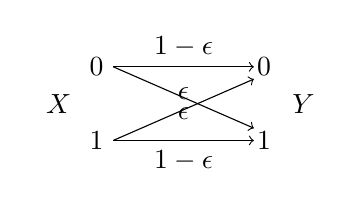
\begin{tikzpicture}[place/.style={inner sep=1pt}]
\matrix
{
    & \node(a1){0};  &    [18mm]     & \node[place](a2){0};        \\
\node{$X$}; &          &              &        &  \node{$\,\, Y$};            \\
    & \node(a3){1};  &             & \node[place](a4){1};        \\
};
\draw[->] (a1.east) --node[above]{$1-\epsilon$} (a2.west);
\draw[->] (a3.east) --node[above]{$\epsilon$} (a2.south west);
\draw[->] (a1.east) --node[below]{$\epsilon$} (a4.north west);
\draw[->] (a3.east) --node[below]{$1-\epsilon$} (a4.west);
\end{tikzpicture}
\end{center}
\caption{二元对称信道}\label{fig:binary_symmetric_channel}%BSC
\end{figure}
\item 二进制删除信道,$I(X;Y)=H(Y)-H(\epsilon)$。 由 "Entropy over disjoint mixture" 得
 $H(Y)=(1-\epsilon)H(X)+H(\epsilon)\Rightarrow I(X;Y)=(1-\epsilon)H(X)\leq 1-\epsilon$,当$X\sim Berm({1\over 2})$时取等号。

\begin{figure}[!ht]
\begin{center}
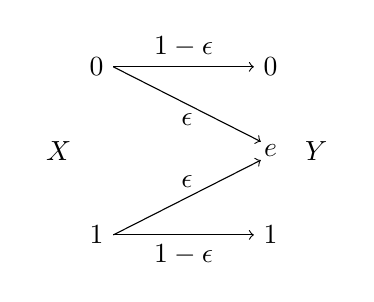
\begin{tikzpicture}[place/.style={inner sep=1pt},row sep=6mm]
\matrix
{
    & \node(a1){0};  &    [18mm]     & \node(a2){0};        \\
\node{$X$}; &          &              &   \node[place](a5){$e$};     &  \node{$\,\, Y$};            \\
    & \node(a3){1};  &             & \node(a4){1};        \\
};
\draw[->] (a1.east) --node[above]{$1-\epsilon$} (a2.west);
\draw[->] (a1.east) --node[below]{$\epsilon$} (a5.north west);
\draw[->] (a3.east) --node[above]{$\epsilon$} (a5.south west);
\draw[->] (a3.east) --node[below]{$1-\epsilon$} (a4.west);
\end{tikzpicture}
\end{center}
\caption{二进制删除信道}\label{fig:binary_erasure_channel}
\end{figure}

\end{enumerate}
\item 对称信道的信道容量:
设$Q$有$K$行$J$列,则信道容量 $C = \log J - H(Y|a_k)$,其中 
$$
H(Y|a_k) = -\sum_{j=1}^J q(b_j | a_k) \log q(b_j | a_k)
$$
由 $Q$的各行互为排列可知 $H(Y|a_k)$ 与$k$无关。
当输出分布等概时取到$C$。
\item 离散无记忆信道的信道容量定理

对于信道转移矩阵为$Q$的离散无记忆信道,输入分布 $p^*(x) = (p^*(a_1), p^*(a_2), \dots, p^*(a_K))$ 能使互信息达到最大的充要条件是, 存在常数$C$, 使得在此分布下:
\begin{align*}
    I(X = a_k; Y) = C & ; \text{ as } p^*(a_k) > 0 \\
    I(X = a_k; Y) \leq C & ; \text{ as } p^*(a_k) = 0 
\end{align*}
其中 $I(X = a_k; Y) = \sum_{j=1}^J q(b_j | a_k) \log \frac{q(b_j | a_k)}{p(b_j)}$ 为$ a_k$ 与 $Y$ 的互信息, $C$为信道容量。

\item 准对称信道的信道容量定理

准对称信道, 输入分布为等概时达到信道容量。

\item 一般 DMC 信道在$K = J$条件下的信道容量求解。

$K+1$ 个方程, $K+1$ 个未知数($C$和 $p(b_j), j = 1, 2, \dots, K$)

\begin{align}
\label{eq:IC}    I(X = a_k; Y) = C, & k = 1, 2, \dots, K \\
\label{eq:normalization}   \sum_{j=1}^J p(b_j) = 1 &
\end{align}

\eqref{eq:IC} 式变换得到:
\begin{equation*}
    H(Y | X = a_k) = \sum_{j=1}^K q(b_j | a_k) \beta_j; \beta_j = C + \log p(b_j), k = 1, 2,\dots K
\end{equation*}
即:
$$
\bm{Q} \begin{bmatrix} \beta_1 \\ \beta_2 \\ \vdots \\ \beta_K \end{bmatrix} 
    = - \begin{bmatrix} H(Y|X = a_1) \\ H(Y|X = a_2) \\ \vdots \\ H(Y|X = a_3) \end{bmatrix} 
$$
由此解出 $\beta_j$ 后将 $p(b_j) = 2^{\beta_j - C}$ 代入~\eqref{eq:normalization} 式中解出
$ C =\log\left(\sum_{j=1}^K 2^{\beta_j}\right)$
\item 多符号离散无记忆信道的信道容量
$ \bm{x} = x_1x_2\dots x_N, \bm{y} = y_1y_2\dots y_N$, 转移概率矩阵为
$ q(\bm{y} | \bm{x}) = \prod_{n = 1}^N q(y_n | x_n)$,
可以证明 $I(\bm{X}; \bm{Y}) \leq \sum_{n = 1}^N I(X_n; Y_n)$, 当信源离散无记忆时可取到等号。
因为当信源离散无记忆时,有不等式 $I(\bm{X}; \bm{Y}) \geq \sum_{n = 1}^N I(X_n; Y_n)$。
对于多符号的情形, 信道容量定义为:
$$
C = \lim_{N \to \infty} {1 \over N} \max_{p(\bm{X})} I(\bm{X}; \bm{Y})
$$
\item 输出分布的唯一性:最佳分布导致相同的输出分布,任何导致这一输出分布的输入分布都是最佳分布。
\item 组合信道
\begin{enumerate}[label=(\alph*)]
    \item 级联的独立信道, 总的转移概率矩阵 $Q$ 为各级联信道转移概率矩阵之积
    \item 输入并接的信道:输入相同的$X$,输出不同的 $Y_1, Y_2, \dots $, 构成随机矢量$Y$。
    互信息 $ I(X;Y) = I(X; Y_1) + I(X; Y_2\dots Y_N | Y_1) \geq I(X; Y_1)$, 所以
    $ \max_n C_n \leq C $
    \item 并用信道:$X$ 和 $Y$ 由彼此独立的 $N$ 个信道传输。
    $Y_n = f_n (X_n)$, 当 $X_n$ 彼此独立时, 有 $ I(X; Y) = \sum_{n=1}^N I(X_n; Y_n)$
    因此 $C = \sum_{n=1}^N C_n$
    \item 和信道: 随机使用 $N$个信道中的一个,设$\bm{P} = [p_1, \dots, p_n]$ 为随机使用各个信道的概率。
    则 $I(X; Y) = \sum_{i=1}^N p_i (I(X_i; Y_i)-\log p_i)$($\log p_i $ 是由于输出分布带$p_i$,在原来互信息的定义式中被提出来了)。
    $ C = \max_{\bm{P}} \sum_{i=1}^N p_i (C_i - \log p_i)$, 用 Lagrange 乘子法求解得到:
$ C = \log \sum_{i=1}^N 2^{C_i}$ 且 信道使用概率为 $p_i = 2^{C_i - C}$
\end{enumerate}
\item 连续无记忆加性噪声信道:$ Y = X + Z$, 可以求出微分熵 $h(Y|X) = h(Z)$,
因此$I(X; Y) = h(Y) - h(Y|X) = h(Y) - h(Z)$。
若输入信号的均值为零, 平均功率为 $P_S$, 则信道容量费用函数为:
$$C(P_S) = \max_{p(x)}\{h(Y):\E[X^2] = P_S\} - h(Z)$$

若 $Z$ 是零均值,方差为$P_N$ 的高斯噪声,则输出信号的方差为 $\E[Y^2] = P_S + P_N$。
我们知道,对于给定方差约束的随机变量,最大微分熵的分布是高斯分布,因此当$Y$为高斯分布时,$h(Y)$ 最大,从而达到最大的信道容量, 此时输入信号 $X = Y - Z $ 也是高斯分布。
\begin{align*}
C(P_S)  & = {1 \over 2} \log[2\pi e(P_S + P_N)] - {1 \over 2} \log[2\pi e P_N] \\
  & = {1\over 2} \log\left(1 + {P_S \over P_N}\right)
\end{align*}
\item 并联的连续信道: $X=(X_1X_2\dots X_n), Y=(Y_1Y_2\dots Y_n)$。
每个 $Y_i = X_i + Z_i$。$Z_i$ 为高斯分布,功率为 $P_{N_n}$,
根据前一节的结论,当每个信道功率$P_{S_n}$给定时,该信道的容量为
${1\over 2} \log(1+{P_{S_n} \over P_{N_n}})$。设各信道的输入信号之间相互独立,给定
输入信号的总功率约束为 $\sum_{n=1}^N \E[X_n^2] = P_S$,则并联信道的容量为:
$$
C(P_S) =\sum_{k=1}^n {1\over 2} \log(1+{P_{S_k} \over P_{N_k}}),\, s.t. \sum_{k=1}^n P_{S_k} = P_S
$$
使用 Lagrange 乘子法求解得到当 $P_{N_k} < \lambda' \triangleq \displaystyle{ P_S + \sum_{k=1}^n P_{N_k} \over N}$ 时
$P_{S_k} = \lambda' - P_{N_k}$,否则置 $P_{S_k} = 0 $(不使用该信道),并重新计算 $\lambda'$(重新进行功率分配)。

\item 限带加性高斯白噪声信道 (AWGN) $ y(t) = x(t) + z(t) $

噪声的功率谱密度为  
\begin{equation}
S_N(f)=\begin{cases}
0 & \textrm{if} |f|>W\\
\frac{N_0}{2} & \textrm{if} |f|<W
\end{cases}
\end{equation}
作 Fourier 反变换得到 自相关函数为 $R(\tau) = N_0 W \frac{\sin(2\pi W\tau)}{2\pi W\tau}$,
若每隔$\Delta t = \frac{1}{2W}$ 的时间间隔采样,则采样点上的噪声相互独立。

根据Nyquist-Shannon 采样定理,每隔$\frac{1}{2W}$ 可以完全恢复信号,因此原信号可等效表示成
$2WT$间隔为$\frac{1}{2W}$的采样值$X_1, X_2,\dots, X_N(N=2WT)$, 每次采样值通过一个AWGN 信道, 噪声功率为
$\frac{N_0WT}{2WT} = \frac{N_0}{2}$, 信号功率为 $\frac{P_S T}{2WT} = \frac{P_S}{2W}$。
则容量费用函数为:
\begin{align}\notag
C(P_S) & = \lim_{T \to \infty} \frac{1}{T} \frac{1}{2} \sum_{n=1}^{2WT} \log\left(1+ \frac{P_S/(2WT)}{N_0/2}\right) \\
\label{eq:shannon} & = W \log(1 + \frac{P_S}{N_0 W})
\end{align}
\eqref{eq:shannon} 即Shannon 公式。

\end{enumerate}

\appendix
\begin{enumerate}
    \item Entropy over disjoint mixture
    
    Let $X_1$ and $X_2$ be discrete random variables and $X$ be defined as 
    $$
    X = \begin{cases}
        X_1 & \text{ with probability } \alpha \\
        X_2 & \text{ with probability } 1 - \alpha 
    \end{cases}
    $$
    Then $H(X) = \alpha H(X_1) + (1-\alpha) H(X_2) + h(\alpha)$

\end{enumerate}
\end{document}





